\documentclass[11pt]{article}

\usepackage[margin=1in]{geometry}
\usepackage{booktabs}
\usepackage{array}
\usepackage{longtable}
\usepackage{hyperref}
\usepackage{xcolor}
\usepackage{tikz}
\usepackage{amsmath}
\usepackage{fancyhdr}
\usepackage{caption}
\usetikzlibrary{arrows.meta,positioning,shapes.geometric,fit}

\hypersetup{
  colorlinks=true,
  linkcolor=blue!60!black,
  urlcolor=blue!60!black,
  citecolor=blue!60!black
}

\pagestyle{fancy}
\setlength{\headheight}{14pt}
\fancyhf{}
\lhead{Disentangled Language Representation}
\rhead{Nikit Phadke}
\cfoot{\thepage}

\newcommand{\code}[1]{\texttt{\detokenize{#1}}}
\newcommand{\score}[1]{\ensuremath{#1}}
\newcommand{\pass}{\textsc{pass}}
\newcommand{\fail}{\textsc{fail}}

\title{\textbf{Disentangled Language Representation:}\\
From Motif Vectors to Causal Process IR}
\author{Nikit Phadke}
\date{June 2026}

\begin{document}
\maketitle

\begin{abstract}
This paper reports a sequence of eight experiments on Disentangled Language
Representation (DLR). The central claim is not that all language can be
compressed into 32 dimensions. Rather, natural language can be decomposed into
multiple layers: a low-dimensional structural motif basis, typed role and
transition frames, causal frame graphs, and process-level trace diagnoses with
latent preconditions. Early experiments show that a 32-dimensional motif vector
can group paraphrases, idioms, and cross-lingual expressions more cleanly than a
surface lexical baseline. Later experiments show why motif vectors alone are
insufficient: they miss role inversion, authority legitimacy, temporal status,
hidden invariants, and local-versus-global success. The final experiments move
from sentence similarity to trace diagnosis. Synthetic multi-event traces are
compiled into ProcessIR objects that identify false terminal states, violated
invariants, authority failures, reconciliation failures, decay sources, and
latent structural preconditions. Across the implemented benchmark suite, DLR
progresses from semantic similarity scoring to a typed causal intermediate
representation for structural language understanding.
\end{abstract}

\section{Introduction}

Modern embedding systems represent utterances as high-dimensional vectors that
mix structure, parameters, bindings, and expression into one space. This is
useful for semantic retrieval, but it makes a different question difficult:
what structural process does an utterance describe?

For example, \emph{He was fired from his job}, \emph{He was given the axe}, and
\emph{Le han dado la puerta} differ in surface form, idiom, and language, yet
they describe the same structural event: an authority removes an agent from an
institutional role boundary. Conversely, \emph{The bank approved my loan} and
\emph{The bank rejected my loan} share most words and entities, but differ in
outcome polarity inside the same permission-gate schema.

The DLR project tests whether language can be decomposed into:

\begin{enumerate}
  \item a 32-dimensional structural motif basis;
  \item scalar parameters such as intensity, urgency, polarity, and confidence;
  \item entity and role bindings;
  \item typed transitions, authority, boundary, invariant, and process status;
  \item causal graphs and process traces.
\end{enumerate}

The experiments began as sentence-pair similarity tests and evolved into
process diagnosis benchmarks. This paper presents the implementation and
results of DLR-1 through DLR-8.

\section{Motif Basis}

The structural vocabulary uses 32 universal motifs grouped into six families.
These motifs are not intended to encode every fact about language. They provide
a basis for structural skeletons, while parameters, bindings, expressions,
frames, and graphs carry the rest of the meaning.

\begin{table}[h]
\centering
\caption{The 32 motif basis.}
\small
\begin{tabular}{p{0.18\linewidth}p{0.72\linewidth}}
\toprule
Group & Motifs \\
\midrule
Existence & State, Transition, Invariant, Identity, Boundary, Terminal State, Decay \\
Persistence & Storage, Addressing, Replication, Synchronization \\
Intelligence & Representation, Feedback, Prediction, Search, Model, Compression, Optimization, Explore/Exploit, Self-Reference \\
Structure & Composition, Hierarchy, Modularity, Abstraction, Emergence \\
Allocation & Scarcity, Queue, Scheduling \\
Coordination & Communication, Authority, Reconciliation, Negotiation \\
\bottomrule
\end{tabular}
\end{table}

\section{Representation Evolution}

DLR intentionally became more structured over time. Table
\ref{tab:ir_evolution} summarizes the progression.

\begin{longtable}{p{0.12\linewidth}p{0.31\linewidth}p{0.45\linewidth}}
\caption{Evolution of the DLR representation.}
\label{tab:ir_evolution}\\
\toprule
Stage & Object & New capability \\
\midrule
\endfirsthead
\toprule
Stage & Object & New capability \\
\midrule
\endhead
DLR-1 & Motif vector & Tests whether paraphrases and idioms share a structural skeleton. \\
DLR-2 & Typed frame score & Separates same schema from opposite outcome and detects polysemy. \\
DLR-3 & StructuralIR & Adds role slots, transition family, polarity, constraints, and expected relation labels. \\
DLR-4 & Robust StructuralIR & Adds confidence, ambiguity, candidate frames, negation, modality, and pragmatics. \\
DLR-5 & Adversarial IR & Adds parse modes, authority legitimacy, event status, invariant status, process scope, and composite frame graphs. \\
DLR-6 & Causal Frame Graph & Adds typed causal node roles and typed causal edges. \\
DLR-7 & ProcessIR & Diagnoses timestamped multi-event traces with false terminal states and root causes. \\
DLR-8 & ProcessIR plus latent conditions & Adds hidden preconditions, latent nodes, and boundary/identity/decay diagnosis. \\
\bottomrule
\end{longtable}

\begin{figure}[h]
\centering
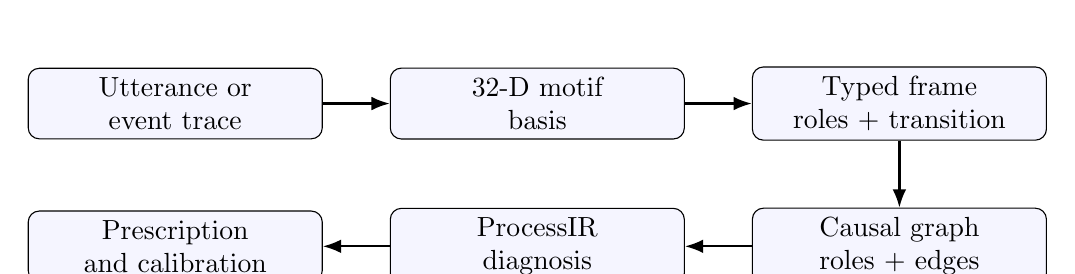
\begin{tikzpicture}[
  node distance=0.85cm,
  box/.style={draw, rounded corners, align=center, minimum height=0.82cm, text width=3.5cm, fill=blue!4},
  arr/.style={-Latex, thick}
]
\node[box] (u) {Utterance or\\event trace};
\node[box, right=of u] (motif) {32-D motif\\basis};
\node[box, right=of motif] (frame) {Typed frame\\roles + transition};
\node[box, below=of frame] (graph) {Causal graph\\roles + edges};
\node[box, left=of graph] (process) {ProcessIR\\diagnosis};
\node[box, left=of process] (rx) {Prescription\\and calibration};
\draw[arr] (u) -- (motif);
\draw[arr] (motif) -- (frame);
\draw[arr] (frame) -- (graph);
\draw[arr] (graph) -- (process);
\draw[arr] (process) -- (rx);
\end{tikzpicture}
\caption{DLR moves from surface utterances to typed process diagnosis.}
\end{figure}

\section{Experimental Suite}

The experiments are synthetic and deterministic. They are designed as
falsification probes, not as claims of broad corpus performance. The purpose is
to test whether the representation has the right failure modes.

\begin{table}[h]
\centering
\caption{Benchmark categories.}
\small
\begin{tabular}{p{0.12\linewidth}p{0.74\linewidth}}
\toprule
Category & Purpose \\
\midrule
A-B & Same structural frame across expression, idiom, and language. \\
C-F & Opposite outcomes, polysemy, gate schemas, and polarity-aware frames. \\
G-H & Role inversion and invalid authority. \\
I-M & Active/passive, ambiguity, context dependence, negation, modality, sarcasm. \\
N-S & Adversarial IR falsification: composite metaphors, deceptive authority, invariant violations, temporal ambiguity, local/global success. \\
T-X & Typed causal graphs for authority, invariant, completion, and terminal outcome. \\
Y1-Y5 & Timestamped process traces with false terminal states and root-cause diagnosis. \\
Z1-Z5 & Hidden preconditions: boundary decay, stale representations, identity aliasing, hidden queues, stale replicas. \\
\bottomrule
\end{tabular}
\end{table}

\section{Scoring}

The early DLR experiments use cosine similarity over motif vectors. Later
experiments add frame and graph channels:

\begin{itemize}
  \item motif similarity;
  \item transition family and transition type compatibility;
  \item role assignment, authority, and boundary compatibility;
  \item outcome and state delta compatibility;
  \item causal node recall and causal edge recall;
  \item root-cause recall;
  \item false-terminal and latent-condition detection.
\end{itemize}

For DLR-3 and later, polarity contributes only inside compatible transition
families. This avoids giving high scores to examples such as employment firing
and weapon firing merely because both include a forceful transition.

\section{Results}

\subsection{DLR-1 and DLR-2: Motif and Typed Frame Similarity}

The first experiments validated the basic distinction between lexical surface
similarity and structural similarity. In categories A and B, motif vectors
clustered paraphrases and idioms. In category C, typed polarity reduced the
score for approval versus rejection despite shared words.

\begin{table}[h]
\centering
\caption{Early similarity results.}
\small
\begin{tabular}{lrrrp{0.43\linewidth}}
\toprule
Category & Baseline & Motif & Typed frame & Interpretation \\
\midrule
A & 0.0297 & 0.9988 & 0.9447 & Hunger variants share a frame. \\
B & 0.1024 & 1.0000 & 1.0000 & Job termination idioms share a frame. \\
C & 0.6316 & 0.5386 & 0.3434 & Loan approval and rejection split by outcome. \\
D & 0.5161 & 0.4528 & 0.2807 & Hunger polysemy does not collapse blindly. \\
E & 0.3403 & 0.5325 & 0.2768 & \emph{Fired} polysemy is separated by frame type. \\
F & 0.3230 & 0.6678 & 0.5263 & Gate schemas align while polarity remains explicit. \\
\bottomrule
\end{tabular}
\end{table}

\subsection{DLR-3 through DLR-8}

\begin{table}[h]
\centering
\caption{Summary of later experiment results.}
\small
\begin{tabular}{lrrrrp{0.34\linewidth}}
\toprule
Stage & Cases & Passed & Accuracy & Confidence & Main finding \\
\midrule
DLR-3 & 51 & 51 & 1.0000 & -- & StructuralIR handles roles, authority, and polarity. \\
DLR-4 & 13 & 13 & 1.0000 & 0.7615 & Ambiguity and modality can be calibrated. \\
DLR-5 & 13 & 12 & 0.9231 & 0.6746 & Adversarial IR reveals one useful authority/invariant confusion. \\
DLR-6 & 10 & 10 & 1.0000 & 0.7950 & Typed causal graphs separate five causal patterns. \\
DLR-7 & 5 & 4 & 0.8000 & 0.8200 & ProcessIR detects all false terminal states; one high-confidence decay miss. \\
DLR-8 & 5 & 5 & 1.0000 & 0.8080 & Latent hidden preconditions are recovered in all Z traces. \\
\bottomrule
\end{tabular}
\end{table}

\begin{figure}[h]
\centering
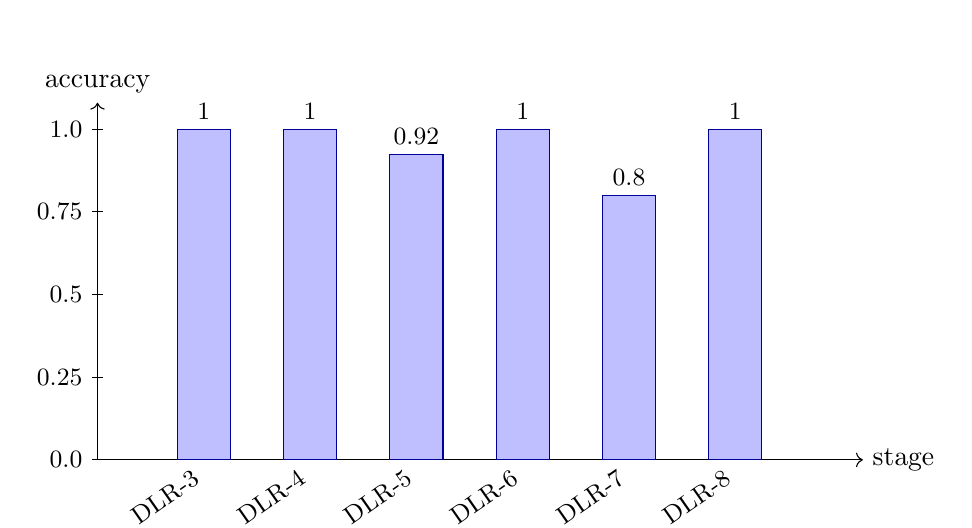
\begin{tikzpicture}[x=1.35cm,y=4.2cm]
  \draw[->] (0,0) -- (7.2,0) node[right] {stage};
  \draw[->] (0,0) -- (0,1.08) node[above] {accuracy};
  \foreach \y/\lab in {0/0.0,0.25/0.25,0.5/0.5,0.75/0.75,1/1.0} {
    \draw (-0.05,\y) -- (0.05,\y);
    \node[left] at (-0.05,\y) {\small \lab};
  }
  \foreach \x/\name/\val in {1/DLR-3/1.0,2/DLR-4/1.0,3/DLR-5/0.9231,4/DLR-6/1.0,5/DLR-7/0.8,6/DLR-8/1.0} {
    \draw[fill=blue!25,draw=blue!60!black] (\x-0.25,0) rectangle (\x+0.25,\val);
    \node[below,rotate=35,anchor=east] at (\x,-0.03) {\small \name};
    \node[above] at (\x,\val) {\small \pgfmathprintnumber[fixed,precision=2]{\val}};
  }
\end{tikzpicture}
\caption{Stage accuracy from StructuralIR validation through hidden precondition diagnosis.}
\end{figure}

\subsection{False Terminals and Latent Preconditions}

The process-level experiments are the strongest evidence for why single-frame
sentence similarity is insufficient. DLR-7 and DLR-8 show that a local subsystem
can report success while the parent process has not reached a valid terminal
state. DLR-8 further shows that the root cause may be latent: not an event in
the trace, but a hidden boundary, identity, representation, queue, or replication
condition inferred from the trace.

\begin{table}[h]
\centering
\caption{Process-level diagnostic results.}
\begin{tabular}{lrrrrr}
\toprule
Stage & Node recall & Edge recall & Root cause & False terminal & Overconf. fail \\
\midrule
DLR-7 & 0.9667 & 0.9500 & 0.9000 & 1.0000 & 0.2000 \\
DLR-8 & 1.0000 & 1.0000 & 1.0000 & 1.0000 & 0.0000 \\
\bottomrule
\end{tabular}
\end{table}

\begin{table}[h]
\centering
\caption{DLR-8 hidden precondition categories.}
\small
\begin{tabular}{p{0.11\linewidth}p{0.34\linewidth}p{0.2\linewidth}p{0.2\linewidth}}
\toprule
Cat. & Hidden condition & Latent kind & Motif \\
\midrule
Z1 & Symlink/path alias crosses a declared filesystem boundary. & boundary decay & Boundary, Decay \\
Z2 & Worker uses a stale cached policy snapshot. & stale representation & Representation \\
Z3 & Email canonicalization collapses two identities. & identity alias & Identity \\
Z4 & Schedule success hides an execution backlog. & hidden queue & Queue, Scheduling \\
Z5 & Read replica diverges from primary inventory state. & replication divergence & Replication, Synchronization \\
\bottomrule
\end{tabular}
\end{table}

\section{Examples}

\subsection{Role and Authority}

DLR-3 adds role inversion tests such as:

\begin{quote}
The doctor cleared him for surgery.\\
He cleared the doctor for surgery.
\end{quote}

The motif bag and transition family are similar, but the authority and role
assignment are invalid. The typed IR assigns low role similarity and low final
structural score.

\subsection{Local Success, Global Failure}

In DLR-7, the release incident trace contains:

\begin{quote}
CI passed unit tests. CD marked deployment successful. The release bot closed
the ticket. Health checks then reported a 500 spike.
\end{quote}

The local deploy step is a transition, but the release is not terminal-valid.
The ProcessIR marks the deploy success as a false terminal state, ticket closure
as a premature transition, and health failure as a terminal outcome.

\subsection{Latent Boundary Decay}

In DLR-8, a cleanup tool deletes \code{/tmp/cache}. Later the workspace cache is
missing. The trace does not directly contain the symlink. The gold diagnosis
contains a latent condition:

\begin{quote}
\code{lc_path_alias}: Symlink/path alias made \code{/tmp/cache} resolve into a
workspace-owned cache.
\end{quote}

This is the kind of hidden precondition that a pure event log or sentence
embedding tends to miss.

\section{Discussion}

The experiments support a narrower and stronger version of the initial
hypothesis:

\begin{quote}
The structural skeleton of many utterances can be represented with a compact
motif basis, but robust reasoning requires typed frames, causal graphs, process
state, and latent conditions.
\end{quote}

The 32-dimensional motif vector is useful as a basis, not as a complete
representation. It functions like a low-dimensional physics vocabulary. The
complete representation is closer to an intermediate representation or abstract
syntax tree for events and processes.

\section{Limitations}

The current benchmark is synthetic and deterministic. The parser outputs in
this repository are fixtures, not learned model predictions. Therefore these
experiments validate the representational target and scoring criteria, not yet
an independently trained parser. The next step is to replace hand-authored IR
fixtures with model-generated parses and evaluate whether the same scoring
suite exposes reliable calibration, ambiguity handling, and causal diagnosis.

The reported perfect scores in some stages should not be read as generalization
claims. They indicate that the implemented IR is expressive enough for the
current targeted cases. The useful failures, such as the DLR-5 deceptive
authority versus invariant violation confusion and the DLR-7 agentic decay miss,
are more informative than raw accuracy.

\section{Reproducibility}

The repository includes executable TypeScript experiments and generated JSON
artifacts. The main commands are:

\begin{verbatim}
npm install
npm run typecheck
npm run run:report
npm run run:dlr3
npm run run:dlr4
npm run run:dlr5
npm run run:dlr6
npm run run:dlr7
npm run run:dlr8
\end{verbatim}

The generated reports are:

\begin{itemize}
  \item \code{dlr_results.md}
  \item \code{dlr3_structural_ir.md}
  \item \code{dlr4_parser_robustness.md}
  \item \code{dlr5_adversarial_ir_falsification.md}
  \item \code{dlr6_causal_frame_graph.md}
  \item \code{dlr7_trace_to_causal_ir.md}
  \item \code{dlr8_hidden_preconditions.md}
\end{itemize}

\section{Conclusion}

DLR began with a simple question: can language be factored into a compact
structural skeleton plus parameters, bindings, and expression? The answer from
these experiments is yes, but only if the skeleton is treated as the first layer
of a richer typed IR. Motif vectors group structural paraphrases. Typed frames
separate role, authority, boundary, and outcome. Causal frame graphs distinguish
invalid authority, invariant violation, blocked attempts, and downstream
failure. ProcessIR diagnoses false terminal states in traces. Latent conditions
capture hidden boundary decay, stale representation, identity aliasing, hidden
queues, and replication divergence.

The practical direction is clear: train or prompt parsers to emit calibrated
StructuralIR and ProcessIR objects, then evaluate them with adversarial graph and
trace benchmarks rather than only embedding similarity.

\end{document}
